%----------------------------------------------------------------------
% Problem 2

\begingroup
\allowdisplaybreaks

\newpage
\section{Problem 2}

\textbf{Exercise 5 in Section 2.7}

\subsection{Solution}

Consider a polynomial with degree 19 containing 20 terms such that

\begin{align*}
	y_i = a_0 + a_1 x_i + a_2 x_i^2 + \ldots + a_{19} x_i^{19}
\end{align*}

where elements $x_i \in \bv{x}$ and $y_i \in \bv{y}$ are sampled from $-1$ to $1$ in steps of $0.1$. This problem can be formulated as a discrete linear inverse problem of the form $G\bv{m} = \bv{d}$. The operator $G$ of size $21 \times 20$ is formed as

\begin{align*}
	G = \begin{bmatrix}
		1 & x_1 & x_1^2 & \cdots & x_1^{19} \\
		1 & x_2 & x_2^2 & \cdots & x_2^{19} \\
		\vdots & \vdots & \vdots & \ddots & \vdots \\
		1 & x_{21} & x_{21}^2 & \cdots & x_{21}^{19}
	\end{bmatrix}
\end{align*}

and model parameters $\bv{m} \in \R^{20}$ are the polynomial coefficients. The normal equations are applied as

\begin{align*}
	\bv{m}_{L2} = \left(G^T G\right)^{-1} G^T \bv{y}
\end{align*}

which should ideally result in $a_1 = 1$ and all other coefficients equal zero. Evaluating the normal equations in \MATLAB reveal model parameters that are close but not exact to ideal as shown in figure \ref{fig: prob2 model params}. 

\begin{figure}[h] 
	\centering
	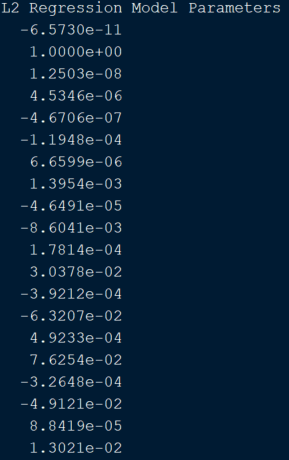
\includegraphics[width=0.45\textwidth]{./images/prob2_model_params.png}
	\caption{Model Parameters}
	\label{fig: prob2 model params}
\end{figure}
\FloatBarrier

While $a_1$ equals one as expected, all other terms are \textit{close to zero, but not exactly zero}. 20 coefficients are far too many for fitting a line, but the result is interesting. Figure \ref{fig: prob2 residuals} shows the residuals in the L2 regression which take an interesting shape.

\begin{figure}[h] 
	\centering
	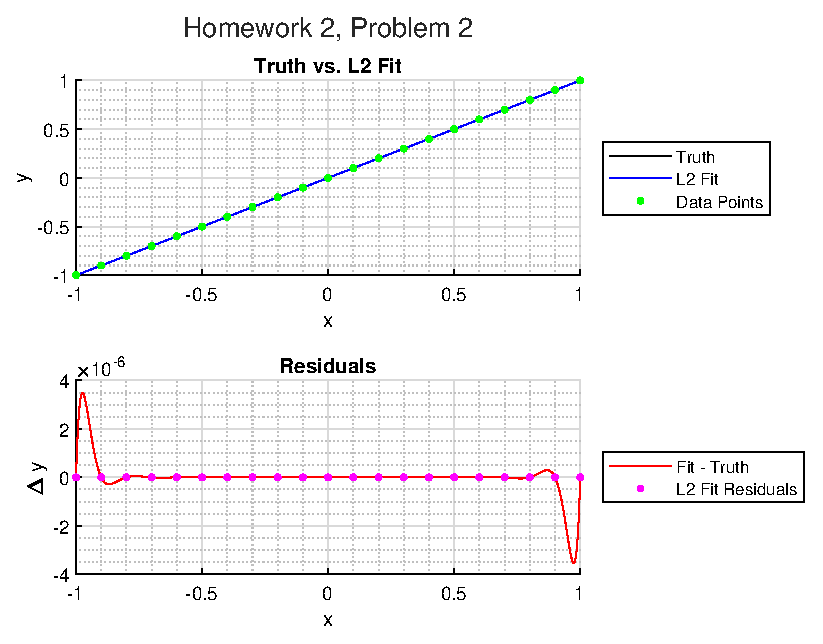
\includegraphics[width=0.8\textwidth]{./images/prob2_1.eps}
	\caption{Data, Fitted Model, and Residuals}
	\label{fig: prob2 residuals}
\end{figure}
\FloatBarrier

This is an extreme example of over-fitting the data. By simple observation of the data, there are 18 extra unnecessary parameters to fit this linear trend. 

